\documentclass[a4paper,titlepage,twoside,12pt,leqno]{article}

\usepackage[]{fontspec}
\usepackage{xltxtra}
\usepackage[monogreek]{xgreek}

\newcommand{\en}[1]{\setlanguage{american}#1\setlanguage{monogreek}} % Για υφενώσεις στα αγγλικά

\defaultfontfeatures{Mapping=tex-text%, Scale=MatchLowercase}
} 

% Γραμματοσειρά
\setmainfont[Mapping=tex-text]{DejaVu Sans}


\usepackage{longtable} % για έναν μεγάλο πίνακα
\usepackage{graphicx, array, blindtext}

%Για την εντολή \caption* και την αφαίρεση του πίνακας 1:
\usepackage{caption}


\begin{document}

%Για την αφαίρεση της αρίθμησης των σελίδων
\pagestyle{empty}


\begin{table}[ht]
\caption*{\huge{Σύντομες οδηγίες εκκίνησης}}
\centering
\begin{tabular}{*{2}{m{0.48\textwidth}}}
\hline

\begin{center}
\emph{Eισαγωγική οθόνη}\\
\resizebox*{0.4\textwidth}{0.3\textwidth}{
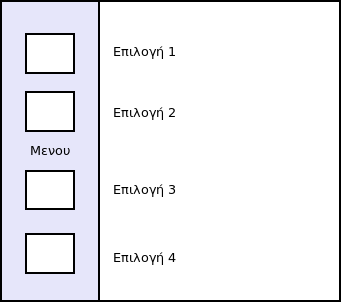
\includegraphics{images/menu.png}}
\end{center} 

& 
Στα αριστερά του παραθύρου φαίνονται τα μενού στα οποία οδηγεί η εφαρμογή. Στα δεξία του παραθύρου φάινονται σημαίες χωρών και πατώντας σε αυτές αλλάζει η γλώσσα της εφαρμογής. Τα εικονίδια στα αριστερά παραμένουν καθ` όλη την διάρκεια εκτέλεσης της εφαρμογής.\\
\hline

\begin{center}
\emph{Μενού παραγγελίας}\\
\resizebox*{0.4\textwidth}{0.3\textwidth}{
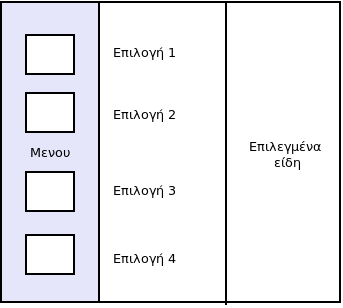
\includegraphics{images/menu_paraggelia.png}}
\end{center} 

& 
Μέσω του μενού παραγγελίας πραγματοποιούνται οι ηλεκτρονικές παραγγελίες. Στα δεξία της οθόνης φαίνονται τα αντικείμενα που έχει επιλέξει ο χρήστης ενώ στο κέντρο φαίνονται τα αντικείμενα τα οποία προσφέρει η καστροπολιτεία. \\
\hline

\begin{center}
\emph{Μενού διαχείρισης τάφρου-πισίνας}\\
\resizebox*{0.4\textwidth}{0.3\textwidth}{
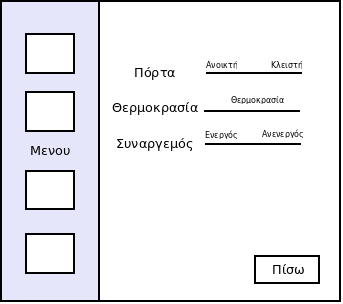
\includegraphics{images/menu_pisina.png}}
\end{center} 

& 
Στο μενού της διαχείρισης της τάφρου-πισίνας ρυθμίζεται η πόρτα του διαμερίσματος, η θερμοκρασία και ο συναγερμός της πισίνας μέσω της αντίστοιχης μπάρας.\\
\hline
 
\end{tabular}
\label{table:getting_started}
\end{table}


\begin{table}[ht]
\centering
\begin{tabular}{*{2}{m{0.48\textwidth}}}
\hline

\begin{center}
\emph{Eισαγωγική οθόνη}\\
\resizebox*{0.4\textwidth}{0.3\textwidth}{
\rule{0.4\textwidth}{0.3\textwidth}}
\end{center} 

& 
Στα αριστερά του πα.\\
\hline


\end{tabular}
\label{table:getting_started_2}
\end{table}



\end{document}
